\section{Kryptographie}

\subsection{Einführung in die Kryptographie}

\begin{remark}
    In diesem Kapitel schauen wir uns die Ziele, Grundbegriffe und Modelle der Kryptologie an.
\end{remark}

\begin{concept}{Zweige der Kryptologie}
    
    Die \textcolor{darkturquoise}{\textbf{Kryptologie}} ist ein Teil der Mathematik, welcher sich mit dem sicheren Übertragen und Speichern von Nachrichten beschäftigt.

    \begin{itemize}
        \item \textcolor{darkturquoise}{\textbf{Kryptographie}}: Die Wissenschaft der Verschlüsselung von Nachrichten (sicheres Speichern und Übertragen) $\rightarrow$ sichere Protokolle und deren Aufbau
        \item \textcolor{darkturquoise}{\textbf{Kryptoanalyse}}: Die Wissenschaft des Entschlüsselns von Nachrichten (wie können Mechanismen der Kryptographie gebrochen werden?) $\rightarrow$ alte, unsichere Protokolle und deren Schwachstellen
    \end{itemize}
\end{concept}

\begin{theorem}{Ziele der Kryptographie}
    Nachrichten sicher übertragen und speichern. \textit{Sicherheit} hat dabei verschiedene Aspekte:
    \begin{itemize}
        \item \textcolor{darkfrog}{\textbf{Confidentiality:}} Nur berechtigte Personen können eine Nachricht lesen. Unberechtigte Personen können die Nachricht zwar sehen, sie aber nicht entziffern, da die Nachricht für sie nur aus einer zufälligen Zeichenfolge zu bestehen scheint.
        \item \textcolor{darkfrog}{\textbf{Integrity:}} Eine Nachricht wird vom Empfänger so empfangen, wie sie vom Sender geschickt wurde. Das heisst, eine unberechtigte Person könnte zwar eine Nachricht abfangen, verändern, und dem Empfänger zustellen. Dieser würde dann aber merken, dass die Nachricht nicht der ursprünglichen Nachricht entspricht und sie daher verwerfen.
        \\ $\rightarrow$ Der Empfänger kann sicher sein, dass die Nachricht nicht verändert wurde.
        \item \textcolor{darkfrog}{\textbf{Authenticity:}} Der Empfänger kann sicher sein, dass eine Nachricht auch wirklich von der Person stammt, von welcher die Nachricht zu kommen scheint. Das heisst, er kann überprüfen, ob der angegebene Absender auch dem tatsächlichen Absender entspricht.
        \item \textcolor{darkfrog}{\textbf{Non-repudiation:}} Wenn eine Person eine Nachricht bekommen hat, kann diese Person nicht abstreiten, dass sie die Nachricht erhalten hat. Das heisst, es kann bewiesen werden, dass sie die Nachricht erhalten hat.
        \item \textcolor{darkfrog}{\textbf{Freshness:}} Alle erhaltenen Nachrichten sind aktuell. Das heisst, ein Attacker könnte zwar eine Nachricht zurückbehalten und später senden, oder eine abgefangene Nachricht duplizieren und zu einem späteren Zeitpunkt noch einmal senden, aber dies würde vom Empfänger bemerkt.
        \item \textcolor{darkfrog}{\textbf{Anonymity:}} Der Absender und/oder Empfänger einer Nachricht bleiben unbekannt.
    \end{itemize}
\end{theorem}


\subsubsection{Model der Kommunikation und Verschlüsselung}

\begin{definition}{Kommunikationsmodel}

    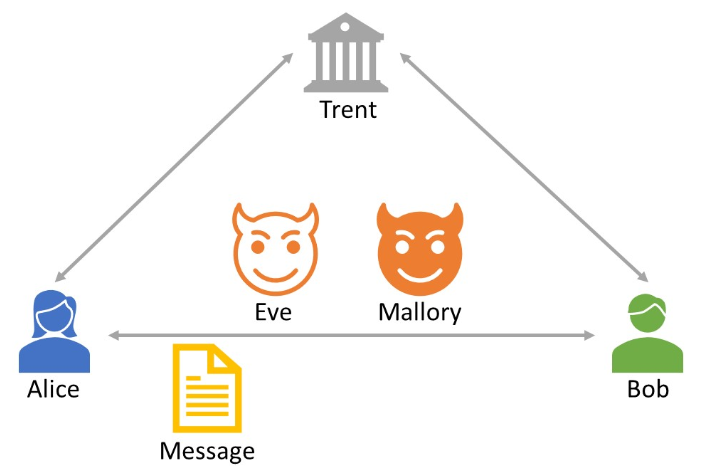
\includegraphics[width=\linewidth]{kommunikationsmodel.png}

    \begin{itemize}
        \item \textcolor{darkblue}{\textbf{Alice}} sendet eine Nachricht an Bob. Dabei sollen die oben genannten Ziele, confidentiality, integrity, authenticity, non-repudiation und freshness erfüllt werden.
        \item \textcolor{darkgreen}{\textbf{Bob}} empfängt die Nachrichten von Allice. Er will überprüfen können, dass die Ziele eingehalten wurden.
        \item \textcolor{darktangerine}{\textbf{Eve}}  ist ein Attacker. Sie kann Nachrichten mitlesen, aber sie nicht verändern.
        \item \textcolor{darkred}{\textbf{Mallory}} ist ein anderer Attacker. Er kann Daten sowohl mitlesen als auch verändern. Er kann auch Nachrichten abfangen und später weitersenden, oder ganz verwerfen. Er kann auch neue Nachrichten generieren.
        \item \textcolor{darkgrey}{\textbf{Trent}} ist eine Drittperson/Instanz, welcher sowohl Alice und Bob vertrauen. Trent unterstützt Alice und Bob bei der sicheren Kommunikation.
    \end{itemize}
\end{definition}

\begin{concept}{Model der Verschlüsselung}
    Um eine vertrauliche Kommunikation zu erreichen, werden Nachrichten vor dem Senden verschlüsselt und nach dem Empfangen wieder entschlüsselt.

    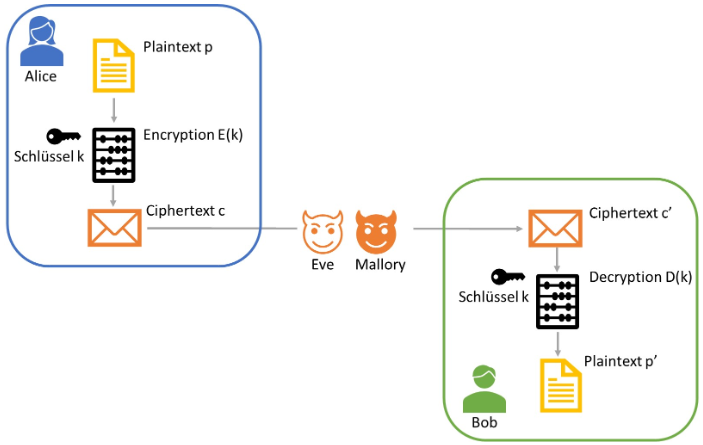
\includegraphics[width=\linewidth]{model_der_verschluesselung.png}

    \begin{itemize}
        \item \textcolor{darkcorn}{\textbf{Plaintext (Klartext):}} Der Plaintext ist der Text, so wie er geschrieben, respektive gelesen werden kann. Er wird mit dem Buchstaben "p" abgekürzt.
        \item \textcolor{darkorange}{\textbf{Ciphertext (Verschlüsselter Text):}} Der Ciphertext ist der Text, welcher durch die Verschlüsselung entsteht. Er wird mit dem Buchstaben "c" abgekürzt.
        \item \textcolor{darkturquoise}{\textbf{Encryption (Verschlüsselung):}} Die Verschlüsselung macht aus dem Plaintext den dazugehörenden Ciphertext. Dazu wird ein Schlüssel verwendet. Die Verschlüsselung kann wie folgt angegeben werden: $c=E[k](p)$. Der Verschlüsselungsalgorithmus selbst ist öffentlich bekannt und kann von allen analysiert werden, um mögliche Schwachstellen zu finden.
        \item \textcolor{darkturquoise}{\textbf{Decryption (Entschlüsselung):}} Die Entschlüsselung macht aus einem Ciphertext den dazugehörenden Plaintext. Dazu wird ein Schlüssel verwendet. Die Entschlüsselung kann wie folgt angegeben werden p' = D[k](c'). Der Entschlüsselungsmechanismus ist öffentlich bekannt und kann von allen analysiert werden, um mögliche Schwachstellen zu finden.
        \item \textcolor{darkpink}{\textbf{Key (Schlüssel):}} Nur mit dem richtigen Schlüssel, kann eine Nachricht richtig entschlüsselt werden. Je nach Art der Verschlüsselung wird derselbe Key für die Verschlüsselung und die Entschlüsselung verwendet (Secret Key Kryptographie) oder es werden unterschiedliche Schlüssel verwendet (Public Key Kryptographie). Damit die Verschlüsselung sicher ist, muss der Schlüssel, welcher für die Entschlüsselung gebraucht wird, geheim bleiben.
    \end{itemize}

    \textbf{Confidentiality} ist erreicht, wenn Eve (und Mallory) den Ciphertext c nicht lesen können. \textbf{Integrity} ist erreicht wenn der von Bob empfangene Plaintext p' dem von Alice gesendeten Plaintext p entspricht, also \textcolor{darkcorn}{\textbf{p' = p}} ist. Authenticity ist erreicht, wenn Bob sicher sein kann, dass die Nachricht von Alice stammt. Non-repudiation ist erreicht, wenn Alice nicht abstreiten kann, dass sie die Nachricht gesendet hat. Freshness ist erreicht, wenn Bob sicher sein kann, dass die Nachricht aktuell ist.
    
\end{concept}

\subsubsection{Attacktypen auf Kryptosysteme}

\begin{remark}
    Die Unterschiede zwischen den Attacken bestehen daraus, auf was der Attacker Zugriff hat.
\end{remark}

\begin{definition}{Ciphertext-only attack}
    Der Attacker kann vom Ciphertext alleine Rückschlüsse auf den Plaintext oder den 
    verwendeten Schlüssel ziehen.
\end{definition}

\begin{definition}{Chosen-ciphertext attack}
    Der Attacker kann Ciphertexte generieren und diese vom System entschlüsseln lassen. 
    Der Attacker bekommt entweder den zum gewählten Ciphertext gehörenden Plaintext 
    (und kann daraus potenziell Rückschlüsse auf den verwendeten Schlüssel machen) 
    oder er bekommt nur Teilinformationen, wie zum Beispiel 
    "Die Entschlüsselung konnte / konnte nicht durchgeführt werden".
\end{definition}

\begin{definition}{Known-plaintext attack}
    Der Attacker kennt sowohl Teile des Plaintext als auch den dazugehörenden Ciphertext (oder zumindest Teile davon). 
    Er kann daraus Rückschlüsse auf andere Plaintexte oder gar den Schlüssel machen.
\end{definition}

\begin{definition}{Chosen-plaintext attack}
    Der Attacker kann Plaintexte wählen, welche er vom System verschlüsseln lassen will. 
    Er erhält dann den dazugehörenden Ciphertext und kann daraus Rückschlüsse auf 
    andere Plaintexte oder gar den Schlüssel machen.
\end{definition}

\begin{definition}{Brute-force attack}
    Der Attacker probiert alle möglichen Schlüssel aus, bis er den richtigen gefunden hat. 
    Dass er den richtigen gefunden hat, erkennt er daran, dass der erhaltene Plaintext sinnvoll erscheint.
\end{definition}

\begin{remark}
    Grundsätzlich können alle Verschlüsselungsalgorithmen mittels brute-force Attacken geknackt werden. 
    Ein wichtiges Evaluationskriterium eines Verschlüsselungsalgorithmus ist also, wie lange eine solche brute-force Attacke im Durchschnitt benötigt. Dieser Anzahl sagt man auch kryptographischer Work Factor.
\end{remark}

\subsubsection{Kryptographischer Work Factor}

\begin{definition}{Work Factor}
    Durchschnittliche Anzahl Versuche, bis der richtige Schlüssel gefunden wird.
    \vspace{2mm}\\
    Der kryptographische Work Faktor kann als Mass der Stärke für eine Verschlüsselung herangezogen werden. Der Work Faktor bezeichnet die durchschnittliche Anzahl Versuche, bis man den richtigen Schlüssel bei einer Brute Force Attacke gefunden hat.
    \vspace{2mm}\\
    Ein Algorithmus hat dann einen genügend grossen Work Faktor wenn es unrealistisch ist, den richtigen Schlüssel per brute force zu erraten.
\end{definition}

\begin{concept}{Einflussfaktoren auf den Work-Factor}
    \begin{itemize}
        \item \textbf{Verschlüsselungsalgorithmus:} Je nach verwendetem Algorithmus ist die Berechnung des Work Faktors anders. Wir werden in den entsprechenden Kapiteln jeweils den dazugehörenden Work Faktor auflisten.
        \item \textbf{Schlüssellänge:} Grundsätzlich gilt: Je länger der Schlüssel, desto höher der Work Faktor
        \item \textbf{Zufälligkeit des Schlüssels:} Der Work Faktor von einem Algorithmus mit einem Schlüssel fixer länge, ist dann maximal, wenn alle Schlüssel gleich wahrscheinlich sind. Sind die Schlüssel nicht gleich wahrscheinlich, wird der Attacker zuerst die wahrscheinlicheren Schlüssel ausprobieren und so durchschnittlich weniger Schlüssel ausprobieren müssen, bis er den richtigen Schlüssel gefunden hat. Daher ist es sehr wichtig, dass die gewählten Schlüssel immer zufällig sind.
    \end{itemize}
\end{concept}

\begin{formula}{Berechnung des Work-Factors}
    als Hilfe zur Berechnung erfindet man ein unrealistisch schnelles System, welches $10^9$ Chips hat, welcher jeder in $10^{-12}s$ einen Schlüssel ausprobieren kann.
    \vspace{2mm}\\
    durchschn. Zeit je nach grösse Work-Factor (Schlüssellänge):
    \begin{itemize}
        \item $2^{64}$: $1.8 \cdot 10^{-2}$ Sekunden
        \item $2^{96}$: $7.9 \cdot 10^7$ s, ca. 2.5 Jahre
        \item $2^{128}$: $3.4 \cdot 10^{17}$ s, ca. $10^10$ Jahre
        \item $2^{256}$: $1.2 \cdot 10^{56}$ s, ca. $10^{48}$ Jahre
    \end{itemize}
    
    Aus der Tabelle ersichtlich: Algorithmen mit Work-Factor > $2^{128}$ als sicher betrachtet werden.
\end{formula}

\begin{remark}
    Den Work-Factor kann man auch in \textbf{bits} darstellen. Ein Work-Factor von $2^{128}$ entspricht einem Work-Factor von 128 bits. ($2^n$ entspricht $n$ bits)
\end{remark}

\subsubsection{Perfect Secrecy}

\begin{remark}
    Unter einem Algorithmus welcher Informationstheoretisch sicher ist, 
    versteht man einen Algorithmus, bei dem man den ursprünglichen Plaintext nicht kennt, 
    auch wenn man alle Schlüssel ausprobiert hat. 
    Dazu sagt man auch der Algorithmus habe perfect secrecy. 
    Aktuell gibt es nur einen einzigen Algorithmus, welcher diese Eigenschaft erfüllt, 
    der One-Time-Pad (auch bekannt unter dem Namen Vernam Cipher).
\end{remark}

\begin{concept}{One-Time-Pad}
    \begin{itemize}
        \item \textbf{Voraussetzung:} Der Schlüssel ist komplett zufällig und genau gleich lang, wie die zu verschlüsselnde Nachricht.
        \item \textbf{Verschlüsselung:}
        Der Plaintext wird mit dem Schlüssel bitweise ver-xor-ed
        $c_j = p_j \oplus k_j \forall j \in \{1, \dots, n\}$
    \end{itemize}

    Zur Erinnerung: Der XOR Operator ist definiert als:
    \begin{center}
        \begin{tabular}{c|c|c}
            $p$ & $k$ & $p \oplus k$ \\
            \hline
            0 & 0 & 0 \\
            0 & 1 & 1 \\
            1 & 0 & 1 \\
            1 & 1 & 0 \\
        \end{tabular}
    \end{center}
\end{concept}

\begin{theorem}{Perfect Secrecy}
    Ein Verschlüsselungsalgorithmus hat perfect secrecy, wenn für alle möglichen Plaintexte $p$ und Ciphertexte $c$ und für alle Schlüssel $k$ gilt:
    \begin{equation}
        P[p|c] = P[p]
    \end{equation}
    Das heisst, dass die Wahrscheinlichkeit, dass ein bestimmter Plaintext $p$ verschlüsselt wurde, gleich gross ist, wie die Wahrscheinlichkeit, dass ein beliebiger Plaintext $p$ verschlüsselt wurde.
\end{theorem}

\begin{corollary}
    Wenn ein Attacker jetzt alle Schlüssel ausprobieren würde, würde er neben vielen offensichtlich falschen Plaintexten auch viele plausible Plaintexte erhalten und wüsste daher nicht, welcher der plausiblen Plaintexte der korrekte ist.
    \vspace{2mm}\\
    Obwohl dies also genau das Verhalten ist, was wir möchten, kommt der One-Time-Pad nur in sehr seltenen Fällen zum Einsatz. Dies liegt daran, dass der Schlüssel
    \begin{itemize}
        \item genau gleich lang wie der zu verschlüsselnde Text sein muss
        \item komplett zufällig sein muss (vollständig zufällige Bitfolge)
        \item vorgängig geheim zwischen Sender und Empfänger ausgetauscht werden muss
        \item nur ein einziges mal verwendet werden darf (sonst ist er nicht mehr vollkommen zufällig und die ganze Sicherheit geht verloren)
    \end{itemize}
\end{corollary}

\begin{concept}{Eigenschaften sicherer kryptographischer Algorithmen}
    Da heute ausser dem One-Time-Pad kein Algorithmus bekannt ist, welcher als informationstheoretisch sicher gilt, werden folgende Eigenschaften für sichere Algorithmen definiert:
    \begin{itemize}
        \item Allgemein bekannt
        \item Keine Fehler bekannt
        \item Work Factor > $2^{128}$
    \end{itemize}
    Daraus lässt sich auch ableiten, dass wir als Noobs keine kryptographischen Algorithmen selber entwickeln/implementieren sollten. Stattdessen soll auf standardisierte Algorithmen zurückgegriffen werden. (Öffentlich verfügbare Libraries)
\end{concept}

\subsection{Kryptographische Hash Funktionen}

\begin{definition}{Kryptographische Hash Funktion} ist eine mathematische Funktion mit folgenden Eigenschaften:
    \begin{itemize}
        \item aus einem beliebig langen Input wird Output mit konstanter Länge generiert
        \item es gibt keine Möglichkeit aus dem Output den Input wieder herzuleiten
        \item unterschiedliche Inputs ergeben mit sehr hoher Wahrscheinlichkeit völlig unterschiedliche Outputs, auch wenn sich die Inputs nur wenig unterscheiden
        \item es ist nicht möglich innert nützlicher Zeit zwei unterschiedliche Inputs zu generieren, welche denselben Output haben
    \end{itemize}

    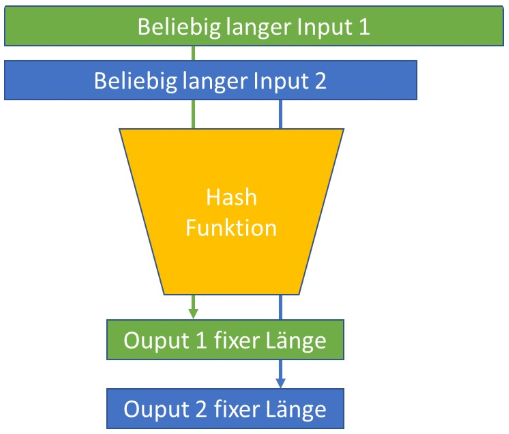
\includegraphics[width=\linewidth]{krypto_hashfunktionen.png}
    
\end{definition}

\begin{formula}{Work Factor}
    Da bei Hash Funktionen der Output weniger lang ist als der Input gibt es keinen Algorithmus, welcher für alle Inputs und Outputs die Eigenschaften 3 und 4 erreicht. Das heisst, es wird immer verschiedene Inputs geben, welche denselben Output generieren. Mit dem Work Faktor kann angegeben werden, wie gross der Aufwand ist, um diese Hash Collisions zu berechnen.

Der Work Faktor in bits einer kryptographischen Funktion entspricht der Hälfte der bits des generierten Outputs.

Auch hier gilt: Für eine sichere Hash Funktion sollte der Work Faktor mindestens 128 bit betragen.    
\end{formula}

\section{Secret Key Cryptography}

\subsection{Principle of Secret Key Cryptography}

\begin{concept}{Secret Key Principle}\\
    The same key is used for encryption and decryption
\end{concept}

\subsection{Block Ciphers}

\begin{definition}{Block Ciphers}\\
    The plaintext is usually not a multiple of the block size.
    \begin{itemize}
        \item Therefore a padding is needed.
        \item Use Block Cipher modes (ECB) / (CBC) for long messages
    \end{itemize}
\end{definition}

% TODO: Add block cipher diagram showing n bits plaintext blocks, key, and block cipher

\subsection{Block Padding (PKCS7)}

\begin{concept}{PKCS7 Padding}\\
    Padding data is used to fill up the final block
    \begin{itemize}
        \item Removal of padding must be easy
        \item PKCS7:
        \begin{itemize}
            \item $n$ bytes must be filled, fill them with byte value $n$
            \item 0 bytes must be filled, add padding block with "10"
        \end{itemize}
    \end{itemize}
\end{concept}

\begin{examplecode}{PKCS7 Example}\\
\begin{lstlisting}[language=text, style=basesmol]
5F 6E 25 A3 36 54 90 0D D4 7F FA 05 05 05 05 05

10 10 10 10 10 10 10 10 10 10 10 10 10 10 10 10
\end{lstlisting}

0 bytes must be filled, add padding block with "10"
\end{examplecode}

\subsection{DES}

\begin{definition}{DES (Data Encryption Standard)}\\
    \begin{itemize}
        \item Key size: 56 bits $\rightarrow$ totally insecure
        \item Brute force attack is still the best attack known
    \end{itemize}
\end{definition}

\subsection{Triple-DES}

\begin{concept}{Triple-DES}\\
    \begin{itemize}
        \item Known-Plaintext Attack (MITM) $\rightarrow$ Cryptographic strength = $2^{112} + 2^{56} \approx 112$ bits
        \item Secure but relatively slow
    \end{itemize}
\end{concept}

% TODO: Add Triple-DES diagram showing P -> DES_E(K1) -> DES_D(K2) -> DES_E(K3) -> C'

\subsection{AES}

\begin{concept}{AES (Advanced Encryption Standard)}\\
    \begin{itemize}
        \item Cryptographic strength = 128 / 192 / 256
        \item Secure and modern standard
        \item Publicly defined
    \end{itemize}
\end{concept}

\subsection{Electronic Code Book Mode (ECB)}

\begin{definition}{ECB Mode}\\
    \begin{itemize}
        \item Same $P$ is always same $C$
        \item Susceptible to replay attacks
        \item Patterns may remain (Pinguin)
    \end{itemize}
\end{definition}

% TODO: Add ECB diagram showing Sender/Receiver with multiple P1->E->C1->D->P1 blocks

\subsection{Cipher Block Chaining Mode (CBC)}

\begin{concept}{CBC Mode}\\
    \begin{itemize}
        \item IV transmitted openly
        \item IV may only be used once
        \item Does not ensure the integrity
    \end{itemize}
\end{concept}

% TODO: Add CBC diagram showing IV chaining with XOR operations

\subsection{Stream Ciphers}

\begin{definition}{Stream Ciphers}\\
    \begin{itemize}
        \item No need to wait for full block
        \item Faster than block ciphers
        \item Most stream ciphers are broken
        \item Can be implemented with block ciphers (OFB, CTR)
        \item Decryption works by reapplying the keystream: $C = P \oplus K \rightarrow P = C \oplus K$
    \end{itemize}
\end{definition}

\subsection{Output Feedback Mode (OFB)}

\begin{concept}{OFB Mode}\\
    Stream cipher with block cipher
\end{concept}

% TODO: Add OFB diagram showing IV, Key, Pseudo-Random Keystream Generator

\subsection{Counter Mode (CTR)}

\begin{concept}{CTR Mode}\\
    \begin{itemize}
        \item Stream cipher with block cipher
        \item Allows for parallel encryption/decryption
    \end{itemize}
\end{concept}

% TODO: Add CTR diagram showing parallel encryption/decryption

\subsection{Security of Stream ciphers}

\begin{remark}
    \begin{itemize}
        \item RC4, GSM A5/1 and A5/2: Considered broken
        \item ChaCha20: Considered secure (Supported by TLS) $\rightarrow$ Today's standard
    \end{itemize}
\end{remark}

\section{Public Key Cryptography}

\subsection{Secure key distribution problem}

\begin{concept}{Key Distribution Problem}\\
    \begin{itemize}
        \item Secret key cryptography only works if the keys are exchange securely
        \item How can we obtain the key from someone unknown?
        \item How do we manage keys for large number of participants?
    \end{itemize}
\end{concept}

\subsection{Principle of public key cryptography}

\begin{definition}{Public Key Cryptography}\\
    \begin{itemize}
        \item \textbf{Public Key} Known to anyone $\rightarrow$ Encryption
        \item \textbf{Private Key} Known to owner $\rightarrow$ Decryption
    \end{itemize}
\end{definition}

\begin{concept}{Properties}\\
    \begin{itemize}
        \item Public and Private key fit together: $D(E(M)) = M$
        \item Private key can't be computed easily from public key
    \end{itemize}
\end{concept}

% TODO: Add public key infrastructure diagram showing Alice, Public Directory, Bob

\subsection{RSA (Rivest-Shamir-Adleman)}

\begin{definition}{RSA Algorithm}\\
    Let $(n, e)$ be RSA public key and $(n, d)$ the corresponding private key. Let $m$ be an integer with $0 \leq m < n$. Then $(m^e \bmod n)^d \bmod n = m$.
    \begin{itemize}
        \item Public Key $(n, e)$
        \item Private Key $(n, d)$
        \item $0 \leq m < n$
        \item $\varphi(n) = (q - 1) \cdot (p - 1)$
    \end{itemize}
\end{definition}

\begin{KR}{RSA Key-Pair Creation}\\
    \paragraph{Step 1: Choose Primes}
    Choose large primes $p, q \rightarrow pq = n$
    
    \paragraph{Step 2: Choose e}
    Choose $e$ so that $\gcd(e,\varphi(n)) = 1$
    
    \paragraph{Step 3: Compute d}
    Compute $d$ so that $ed \bmod \varphi(n) = 1$
\end{KR}

\begin{formula}{RSA Encrypt/Decrypt}\\
    \begin{itemize}
        \item Encrypt: $c = E(m) = m^e \bmod n$
        \item Decrypt: $m = D(c) = c^d \bmod n$
    \end{itemize}
\end{formula}

\subsection{RSA - Attacks}

\begin{definition}{RSA Attack Types}\\
    \textbf{Short message attack (Plain-Text-Attack)}
    \begin{itemize}
        \item Message $m$ is short $\rightarrow$ Ciphertext $c$ easy to decrypt
        \item Prevent by using padding for encryption
    \end{itemize}
    
    \textbf{Low public exponent attack $e$}
    \begin{itemize}
        \item $e$ is "low" and the same message $m$ is sent $e$ times
        \item Prevent by using higher values for value for $e$
    \end{itemize}
    
    \textbf{Common factor attack}
    \begin{itemize}
        \item gcd of two moduli not sharing a common prime factor = 1
        \item gcd of two moduli sharing a common prime factor $\rightarrow$ product of all
        \item If gcd = 1 $\rightarrow$ no common primes, else $p = gcd$
        \item If $p$ has been found: $n/p = q$
    \end{itemize}
\end{definition}

\subsection{Groups}

\begin{definition}{Mathematical Groups}\\
    A group $(G, \circ)$ has the following properties:
    \begin{itemize}
        \item $\circ$ Associative operation: For all $a, b, c \in G$ $(a \circ b) \circ c = a \circ (b \circ c)$
        \item $e$ Neutral element: For all $a \in G$ $e \circ a = a$
        \item $a'$ Inverse element: For all $a \in G$ Exists: $a' \in G \rightarrow a' \circ a = e$
    \end{itemize}
    
    A generator of a group creates all elements when it operates on itself $n$ times.
\end{definition}

\begin{example2}{Example $(Z_7,*)$}\\
    \begin{itemize}
        \item $*$ Associative operation: For all $a, b, c \in G$ $(a * b) * c = a * (b * c)$
        \item $1$ Neutral element: For all $a \in G$ $1 * a = a$
        \item $a'$ Inverse element: For all $a \in G$ Exists: $a' \in G \rightarrow a' \circ a = 1$
    \end{itemize}
    
    3 is a Generator:
    \begin{itemize}
        \item $3 * 1 \bmod 7 = 3$
        \item $3 * 2 \bmod 7 = 6$
        \item $3 * 3 \bmod 7 = 2$
        \item $3 * 4 \bmod 7 = 5$
        \item $3 * 5 \bmod 7 = 1$
        \item $3 * 13 \bmod 7 = 4$
    \end{itemize}
\end{example2}

\subsection{Discrete Logarithm Problem}

\begin{concept}{One-Way Function}\\
    \begin{itemize}
        \item Idea: One-Way function
        \item Direction A: Easy to compute
        \item Direction B: Hard to compute
        \item Example: $(Z_n^*, *)$ for large $n$
    \end{itemize}
\end{concept}

\subsection{Diffie-Hellman key exchange}

\begin{KR}{Diffie-Hellman Protocol}\\
    \paragraph{Setup}
    \begin{itemize}
        \item Alice and Bob agree on large prime $p$
        \item Alice and Bob agree on some generator $g$ of $(Z_p^*, *)$
    \end{itemize}
    
    \paragraph{Key Generation}
    \begin{itemize}
        \item Alice chooses $a$, $(1 < a < p)$
        \item Bob chooses $b$, $(1 < b < p)$
        \item Alice sends $A = g^a \bmod p$
        \item Bob sends $B = g^b \bmod p$
        \item Alice computes $S_A = B^a = (g^b)^a \bmod p$
        \item Bob computes $S_B = A^b = (g^a)^b \bmod p$
    \end{itemize}
    
    \paragraph{Result}
    $S_A = S_B$ is the shared secret only Alice and Bob know.
\end{KR}

% TODO: Add Diffie-Hellman diagram showing Alice/Public/Bob exchange

\begin{remark}
    The secret may not be suitable for to use as a symmetric key:
    \begin{itemize}
        \item Some bits may always be zero or one
        \item The secret may be too long or too short
    \end{itemize}
    
    The secret is put through a key derivation function (KDF) to get the key.
\end{remark}

\subsection{Problems with Diffie-Hellman}

\begin{concept}{DH Limitations}\\
    \begin{itemize}
        \item What if Bob and Alice are not speaking to each other?
        \item Eve can make a Man-in-the-Middle Attack.
        \item Bob and Alice need to be Online.
    \end{itemize}
\end{concept}

\subsection{Integrated Encryption Scheme (IES)}

\begin{concept}{IES}\\
    Solves Offline Problem (of DH)
\end{concept}

\section{Data Integrity and Authentication}

\subsection{Cryptographic Hash Functions}

\begin{definition}{Hash Functions}\\
    A cryptographic one-way hash function maps a variable-length input bit string to a fixed sized output bit string.
\end{definition}

\begin{concept}{Important Properties}\\
    \begin{itemize}
        \item \textbf{Efficient computation}
        \item \textbf{Pseudo-random}
        \item \textbf{Preimage resistance} Given a hash, it is practically impossible to find a massage that produces the hash
        \item \textbf{Collision resistance} It is practically impossible to find any two messages that map to the same hash
    \end{itemize}
    
    A hash function should behave like a random oracle. Different inputs $\rightarrow$ totally unrelated outputs.
\end{concept}

\subsection{Hash Functions}

\begin{remark}
    \begin{itemize}
        \item MD2: Very bad
        \item MD5: Very bad
        \item SHA-1: Getting weaker
        \item SHA-2: considered secure
        \item SHA-3: considered secure (best)
        \item SHA-256: good
    \end{itemize}
\end{remark}

% TODO: Add hash function comparison diagram showing document -> MD5/SHA-1/SHA-2/SHA-3 with different bit outputs

\subsection{Check if a message has been tampered}

\begin{concept}{Message Tampering Detection}\\
    \begin{itemize}
        \item Use a hash function together with a secret key (Message Authentication Code)
        \item Use a hash function together with digital signatures
    \end{itemize}
\end{concept}

\subsection{Authentication with passwords}

\begin{concept}{Password Authentication}\\
    \begin{itemize}
        \item Popular, easy to implement, changeable
    \end{itemize}
\end{concept}

\begin{definition}{Password security problems}\\
    \begin{itemize}
        \item \textbf{Sniffing} Passwords are transmitted in plaintext $\rightarrow$ Prevent with Protected links (TLS)
        \item \textbf{Phishing} Show fake login screen to capture password $\rightarrow$ Prevent with Certificates
        \item \textbf{Online Attacks} Password guessing $\rightarrow$ Prevent with Slowdown / blocking
        \item \textbf{Offline Attacks} Compromises system and gets pw from db $\rightarrow$ Do not save passwords in plaintext
        \item \textbf{Password Re-use} Remove password-strength
    \end{itemize}
\end{definition}

\subsection{Cracking Hashed Passwords}

\begin{KR}{Password Cracking Strategy}\\
    \paragraph{Step 1: Dictionary Attack}
    Try passwords and compute the hash and check if fit matches any hash in the password file
    
    \paragraph{Step 2: Strategic Testing}
    Test strategically with Dictionary attack, Minor variations...
    
    \paragraph{Step 3: Precompiled Attack}
    Compute a huge list of passwords and hashes (beforehand)
\end{KR}

\subsection{Protect password hashes}

\begin{concept}{Salting}\\
    Add a random value called salt before hashing to prevent precompiled attacks.
\end{concept}

% TODO: Add diagram showing ID/Password -> Hash Function with Salt -> Server Password File

\subsection{Collision calculation}

\begin{formula}{Hash Collision Probability}\\
    $n = HashLength$ (in bits)
    \begin{itemize}
        \item Two random Hashes: $2^{n/2}$
        \item Collision with given Hash: $2^{n-1}$
    \end{itemize}
\end{formula}

\subsection{Message Authentication Codes (MAC) = Message Integrity Check (MIC)}

\begin{definition}{MAC Purpose}\\
    The idea is to use a key in addition to the hash function to prevent an attacker from changing the message and calculating a new hash...
\end{definition}

\begin{KR}{MAC Workflow (Using Secret Key Cryptography)}\\
    \paragraph{Step 1} Alice Send document
    \paragraph{Step 2} Bob Apply "Keyed Hash Function" = $MAC_1$
    \paragraph{Step 3} Alice Apply "Keyed Hash Function" = $MAC_2$
    \paragraph{Step 4} Alice Send $MAC_2$
    \paragraph{Step 5} Bob Compare $MAC_1$ and $MAC_2$
\end{KR}

\begin{concept}{HMAC}\\
    HMAC is a concrete implementation of the MAC concept.
    \begin{itemize}
        \item Generate Inner $K_I$ and Outer Key $K_O$
        \item Hash $H(K_I, M) = H_1$
        \item Hash $H(K_O, M) = H_2 = MAC$
        \item Keyed Hash Function: $H(K_O, H(K_I, M))$
    \end{itemize}
\end{concept}

\subsection{Digital Signature}

\begin{KR}{Digital Signature Workflow (Using Public Key Cryptography)}\\
    \paragraph{Step 1} Signer Send document $M$
    \paragraph{Step 2} Verifier Hash document $M \rightarrow H(M) = X$
    \paragraph{Step 3} Signer Hash document $M \rightarrow H(M)$
    \paragraph{Step 4} Signer Encrypt document $H(M) \rightarrow E(H(M))$
    \paragraph{Step 5} Signer Send document $E(H(M))$
    \paragraph{Step 6} Verifier Decrypt document $D(H(M)) \rightarrow H(M) = Y$
    \paragraph{Step 7} Verifier Compare hashes $X == Y$
\end{KR}

% TODO: Add digital signature diagram showing Signer/Verifier workflow

\subsection{Galois Counter mode (GCM)}

\begin{concept}{GCM}\\
    Only encrypting a message doesn't provide Integrity Protection $\rightarrow$ GCM
    \begin{itemize}
        \item Combine Integrity and Encryption
        \item Approach «Encrypt then MAC»
    \end{itemize}
\end{concept}

% TODO: Add GCM diagram showing IV, encryption, authentication process

\subsection{Comparison: MAC vs Digital Signatures}

\begin{concept}{MAC}\\
    \begin{itemize}
        \item Fast and efficient
        \item Receiver must know the secret key
    \end{itemize}
\end{concept}

\begin{concept}{Digital Signatures}\\
    \begin{itemize}
        \item Public key is openly available
        \item En- / Decryption are time intensive
    \end{itemize}
\end{concept}